\documentclass{standalone}

\usepackage{tikz}

\begin{document}

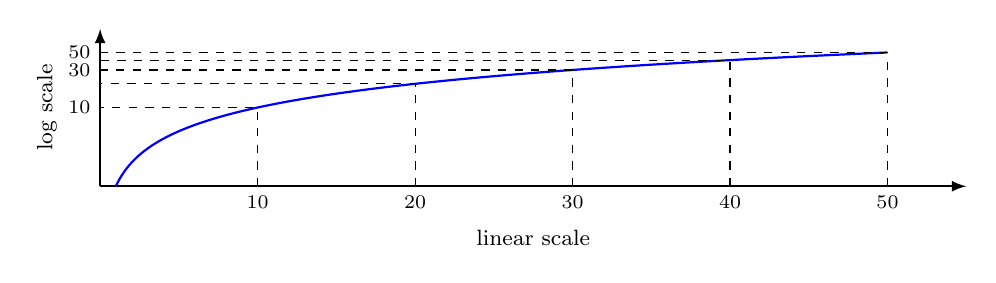
\begin{tikzpicture}
  [>=latex, yscale=1.0, font=\footnotesize]
  \draw [->, thick] (0, 0) -- node [midway, below=12pt] {linear scale} (11, 0);
  \draw [->, thick] (0, 0) -- node [midway, sloped, above=12pt] {log scale} (0, 2.0);

  \draw [draw=blue, thick, domain=0.2:10, samples=400, smooth, variable=\x] plot ({\x}, {log10(5*\x)});

  \foreach \x [evaluate=\x as \y using {int(5*\x)}] in {2,6,10} {
    \draw [dashed] (\x, 0) node [below,font=\scriptsize] {\y} -- (\x, {log10(5*\x)}) -- (0, log10{(5*\x)}) node [left,font=\scriptsize] {\y};
  }

  \foreach \x [evaluate=\x as \y using {int(5*\x)}] in {4,8} {
    \draw [dashed] (\x, 0) node [below,font=\scriptsize] {\y} -- (\x, {log10(5*\x)}) -- (0, log10{(5*\x)});
  }
\end{tikzpicture}

\end{document}

